% IEEE WCNC 2027 -- TWO-PAGE version (2 pp body + references).
% Cut from wcnc-csi.tex (4 pp, canonical) on 2026-09-10 because the EDAS paper
% type enforces a 2-page review manuscript. Same sealed evidence, same claims.
%
% What was cut, and why it is safe:
%  - Fig 1 urllc_relativity and Fig 2 snr_robustness: their numbers are kept in
%    prose (112x; 77-142x across SNR; 54x at table saturation; 0.33 at 3 dB).
%  - Table I (link parameters): folded into the Method paragraph.
%  - Table II(a) (per-seed budget study): folded into prose.
%  - Related work compressed to one paragraph; every citation retained.
%  - The one-sentence pointer to the companion flip paper (dropped for space;
%    it is a forward reference, not a result or a negative disclosure).
% What was NOT cut: the age horizon figure and its per-seed table (the core
% result), the superseded 0.15-threshold disclosure, the curve-resolution limit,
% the diversity-independence caveat, and the scope limits.
\documentclass[conference]{IEEEtran}
\usepackage{cite}
\usepackage{amsmath,amssymb}
\usepackage{graphicx}
\graphicspath{{./build/}}
\usepackage{textcomp}
\usepackage[colorlinks=true,allcolors=blue]{hyperref}

\begin{document}

\title{One CSI-Derived Rate Cannot Serve Every Budget:\\
Budget Overrun and the Age Horizon in 5G Link Adaptation}

\author{\IEEEauthorblockN{Andrew H. Bond}
\IEEEauthorblockA{Department of Computer Engineering\\
San Jos\'e State University, San Jos\'e, CA, USA\\
andrew.bond@sjsu.edu}}

\maketitle
\thispagestyle{empty}
\pagestyle{empty}         % WCNC: no page numbers, headers, or footers

\begin{abstract}
A CSI report drives one rate decision, but different consumers hold that
decision to different error budgets. We measure the mismatch on an NR
LDPC-based link-level simulation. A policy whose achieved BLER sits near an
eMBB budget of $10^{-1}$ overruns a URLLC budget of $10^{-3}$ by a factor of
$112$, at every SNR from cell edge to cell centre. We then calibrate the link
so fresh CSI meets the $10^{-1}$ budget and ask how long a report may be held.
The answer is a few milliseconds at walking pace and a single transmission
interval at moderate mobility, so periodic reporting alone meets the budget
only at the frame minimum. All results come from sealed pre-registered records,
including a superseded relaxed-threshold pilot recomputed here at the
calibrated target.
\end{abstract}

\begin{IEEEkeywords}
CSI feedback, link adaptation, URLLC, outer-loop link adaptation, reliability, 5G NR.
\end{IEEEkeywords}

\section{Introduction}
Adaptive modulation and coding turns a CSI report into a rate decision. The
transmitter selects the highest MCS whose required SINR the report clears, and
the selection is tuned to an error budget. The traffic behind one report does
not share one budget. An eMBB flow tolerates a block error rate of $10^{-1}$; a
URLLC flow tolerates $10^{-3}$ or less. The same decision, from the same report,
on the same channel, is judged against both.

Two quantities stay fixed throughout. The first is the achieved BLER
$\widehat{B}$ of a selection policy. The second is the budget overrun
$\Omega(\beta)=\widehat{B}/\beta$, the achieved BLER in units of the consumer's
budget. $\widehat{B}$ is a property of the policy and the channel. $\Omega$
depends on who is asking.

Two results follow. The first is partly mechanical and we say so: a policy run
near $10^{-1}$ must overrun $10^{-3}$ by about a hundredfold. The second is the
paper's core. With the link calibrated so that fresh CSI meets the $10^{-1}$
budget, the age horizon, the longest a report can be held before the budget is
lost, collapses to a few transmission intervals at $10$\,Hz Doppler and to a
single interval above $50$\,Hz. An earlier exploration at a relaxed threshold
suggested a coherence-proportional law; at the budget itself there is almost no
horizon to scale. The corrections are old, outer-loop link adaptation above all,
and our measurement says when they have stopped being optional.

\section{Method}
\label{sec:method}
\textbf{Substrate.} We use an NR LDPC-based link-to-system simulation at
$3.5$\,GHz with a $1$\,ms TTI. For each MCS of the NR table (TS~38.214
Table~5.1.3.1-1; QPSK--64-QAM, code rates $\ge 1/5$) we measure a block-error
curve $e_m(\gamma)$ with the Sionna 5G LDPC decoder \cite{sionna} over AWGN,
$400$ decoded blocks per point on a $-8$ to $28$\,dB grid at $2$\,dB spacing,
linearly interpolated. The time-domain link draws a per-TTI SNR trace from a
3GPP TR38.901 TDL-A channel ($30$\,ns delay spread, mean SNR $12$\,dB) and
resolves each transmission as
$\mathrm{NACK}(t)\sim\mathrm{Bernoulli}(e_{m}(\gamma(t)))$. Traces are $6000$
TTI for the budget study and $12\,000$ TTI for the age study. Two accuracy
limits bound our claims. At $400$ blocks per point, zero measured errors still
leaves a binomial $95\%$ upper bound near $7.5\times10^{-3}$, so the curves are
trustworthy at $10^{-2}$ and above and any smaller value is an interpolation,
not a count. The mapping also ignores fading within a TTI.

\textbf{System model.} Let $\gamma(t)$ be the true SNR in dB at TTI $t$ and
$\hat{g}(t)$ the estimate the transmitter holds. Fresh CSI reads
$\hat{g}(t)=\gamma(t)+n(t)$ with $n\sim\mathcal{N}(0,\sigma^2)$,
$\sigma=1$\,dB. A report held with period $P$ reads
$\hat{g}(t)=\gamma(t_k)+n(t_k)$ with $t_k=P\lfloor t/P\rfloor$: the estimate
carries the report noise of its issue time and then ages. The certificate
selects, at reference target $\beta_0=10^{-1}$ with backoff $\Delta$,
\begin{equation}
m^\star(\hat{g})=\max\{m:\rho_m(\beta_0)+\Delta\le\hat{g}\},
\label{eq:cert}
\end{equation}
where $\rho_m(\beta)=\min\{\gamma:e_m(\gamma)\le\beta\}$. The achieved BLER is
the empirical NACK rate for the age study and the expected rate
$\tfrac{1}{T}\sum_t e_{m^\star}(\gamma(t))$ for the budget study, whose
$10^{-3}$ scale cannot be resolved by counting at $T{=}6000$.

\textbf{Policies.} The budget-aware policy raises the backoff to
$\Delta=4$\,dB and combines $K{=}3$ diversity branches, independent TDL-A
realizations standing in for frequency or spatial replicas, so a block fails
only if all branches fail. A backoff alone cannot reach $10^{-3}$, because a
single Rayleigh branch spends about $4\%$ of its time in fades too deep for any
MCS. Independence makes the diversity a best case, and the claim rests on a
product rather than a counted deep tail: the per-branch rates sit at the percent
level, where the curves are reliable. The correction of \S\ref{sec:results}
selects $m^\star(\hat{g}(t)+o(t))$ and updates the offset on HARQ feedback,
\begin{equation}
o(t{+}1)=o(t)+\delta_{\mathrm{up}}\,\mathbf{1}[\text{ACK}(t)]
-\delta_{\mathrm{dn}}\,\mathbf{1}[\text{NACK}(t)],
\label{eq:olla}
\end{equation}
with $\delta_{\mathrm{up}}=0.1$\,dB and
$\delta_{\mathrm{dn}}=\delta_{\mathrm{up}}(1-\beta)/\beta$, so the loop settles
where the NACK rate equals $\beta$.

\textbf{Discipline.} Each experiment is pre-registered with bars fixed before
the graded run. Records are content-hashed, graded on seeds disjoint from
design, and kept even when failed, voided or superseded \cite{otcampaigns}.
Review of an earlier draft found the age sweep had used a relaxed $0.15$
threshold while the text claimed $0.10$; that exploration is kept, and
\S\ref{sec:results} reports the calibrated recomputation.

\section{Results}
\label{sec:results}
\textbf{The reliability budget.} Consider one CSI estimate judged under two
budgets. Over three graded seeds of $6000$ TTI with fresh CSI, the naive policy
achieves $\widehat{B}=0.110$ to $0.113$, near its eMBB budget. The URLLC
consumer reads the same value as an overrun of $112\times$. Part of this is
arithmetic and we do not claim otherwise. The measurement adds the exact figure,
the fact that nothing in the scheduler's view flags it, and a feasible remedy:
the budget-aware policy reaches $1.7\times10^{-5}$,
$1.9\times10^{-5}$ and below $10^{-5}$ on the three seeds, meeting the $10^{-3}$
budget with margin. That protection is explicitly specified, a $4$\,dB backoff
and threefold diversity, though we do not quantify its spectral-efficiency cost
here. The overrun is not an artifact of the operating point. A separately sealed
cell sweeping mean SNR from $3$ to $21$\,dB holds the URLLC overrun between
$77\times$ and $142\times$ at every in-range SNR, and still $54\times$ where the
MCS table saturates. Below about $6$\,dB even the eMBB consumer loses its
budget, reaching $\widehat{B}\approx 0.33$ at $3$\,dB, because the lowest MCS is
already too fast for the channel. No margin repairs a certificate whose weakest
format is too aggressive.

\textbf{The age horizon.} At $200$\,Hz Doppler with a $20$-TTI report period the
held estimate is off by $5.7$\,dB on average, aging dominating the $1$\,dB of
report noise, and the naive certificate runs at $\widehat{B}\approx 0.36$
against the $0.10$ budget. OLLA corrects the same held report and holds the
budget, $0.34$ to $0.37$ naive against $0.101$ to $0.102$ corrected over three
sealed seeds.

How long may a report be held? Because the naive fresh policy lands just above
the budget, the age study first calibrates: a fixed backoff
$\Delta_{\mathrm{cal}}=0.5$\,dB, chosen in $0.25$\,dB steps on a disclosed
calibration seed, brings the fresh policy to $\widehat{B}\le 0.09$ at every
Doppler, and all policies then carry it. The horizon is
$P^\star(f_D)=\max\{P:\widehat{B}(P)\le 0.10\}$, and a Doppler at which no
period qualifies is recorded as censored rather than clamped. An exploratory
sweep at a relaxed $0.15$ threshold had suggested
$P^\star\approx 0.18\,T_{\mathrm{coh}}$. It was superseded by the calibrated
experiment reported here, and both records are kept. At the true budget the
answer is starker (Fig.~\ref{fig:age}). Over the three graded seeds
$P^\star$ is $4$, $6$ and $4$ TTI at $10$\,Hz, $2$, $2$ and $3$ at $25$\,Hz, and
$1$ TTI, the frame minimum, at $50$\,Hz and above on every seed. The largest
fresh-CSI $\widehat{B}$ over all Dopplers is $0.078$ to $0.080$, confirming the
calibrated baseline meets the budget, and no Doppler was censored. There is no
room for a proportionality law
because there is almost no horizon to scale. Once the budget is tight, the first
few milliseconds of aging consume it. At $3.5$\,GHz these are modest speeds,
about $3$\,km/h at $10$\,Hz and $15$\,km/h at $50$\,Hz. Below walking pace a
report survives a few TTIs. Above it, periodic reporting meets the budget only
at the frame minimum, so HARQ-driven correction is necessary for any less
aggressive cadence. The coherence-proportional behaviour is real, but it belongs to relaxed
thresholds, where degradation has room to accumulate before the budget is lost.

\begin{figure}[t]
  \centering
  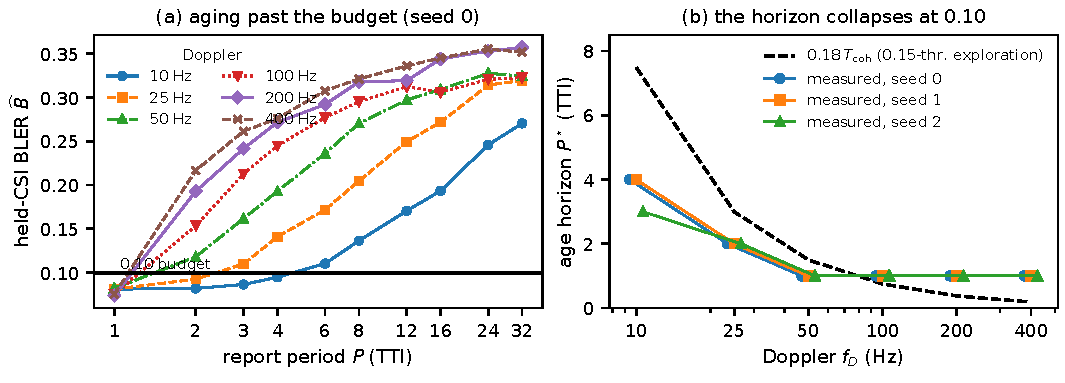
\includegraphics[width=0.80\linewidth]{age_horizon}
  \caption{The age horizon at the true $0.10$ budget (calibrated baseline, three
  sealed graded seeds). (a) Held-CSI BLER against report period; lower is
  better. (b) The horizon collapses to a few TTI at low mobility and to the
  frame minimum above $50$\,Hz.}
  \label{fig:age}
\end{figure}

\section{Related Work and Conclusion}
Link adaptation, CSI aging and outer-loop correction are old subjects. OLLA
\cite{olla} holds an error target under imperfect or stale CSI by adjusting an
SINR offset on HARQ feedback, and it is exactly the correction our age result
makes mandatory. Short-packet analysis \cite{urllc} establishes the reliability
regime where the budget gap lives. NR configures CSI reporting as periodic,
semi-persistent or aperiodic \cite{cqireport}; none adapt the cadence to the
consumer's budget, and our horizon result says how little cadence alone can do
at a tight one. Event-based sampling \cite{sod} we tested only in exploratory
form, and a sealed confirmation attempt was voided by a control check, so we
claim nothing there. For learned CSI feedback \cite{csinet}, the objective gap
it might suggest did not appear in our tests at practical operating points. We
offer no new estimator, scheduler or offset rule. We offer the measurement.

The unit of correctness in link adaptation is not the CSI report. It is the pair
of report and budget. Sized to the consumer's budget, margins and reporting
cadence keep the certificate accurate; sized to a nominal channel they do not,
and the costs are now numbers. The limits are worth stating: one link-to-system
simulation, one TDL-A profile, one MCS table topping at 64-QAM, and values below
$10^{-3}$ limited by curve resolution. Over-the-air HARQ traces are the natural
next step.

\footnotesize
\begin{thebibliography}{1}
\setlength{\itemsep}{0pt plus 0pt}
\setlength{\parsep}{0pt}
\bibitem{olla} A.~Sampath, P.~Sarath~Kumar, and J.~M.~Holtzman, ``On setting reverse link
target SIR in a CDMA system,'' in \emph{Proc. IEEE 47th Veh. Technol. Conf. (VTC)},
vol.~2, 1997, pp.~929--933.
\bibitem{sionna} J.~Hoydis \emph{et al.}, ``Sionna: An open-source library for
next-generation physical layer research,'' arXiv:2203.11854, 2022.
\bibitem{urllc} G.~Durisi, T.~Koch, and P.~Popovski, ``Toward massive, ultrareliable, and
low-latency wireless communication with short packets,'' \emph{Proc. IEEE}, vol.~104,
no.~9, pp.~1711--1726, 2016.
\bibitem{cqireport} 3GPP TS~38.214, ``NR; Physical layer procedures for data,''
v17, clause~5.2, 2022.
\bibitem{sod} M.~Miskowicz, ``Send-on-delta concept: An event-based data reporting
strategy,'' \emph{Sensors}, vol.~6, no.~1, pp.~49--63, 2006.
\bibitem{csinet} C.-K.~Wen, W.-T.~Shih, and S.~Jin, ``Deep learning for massive MIMO CSI
feedback,'' \emph{IEEE Wireless Commun. Lett.}, vol.~7, no.~5, pp.~748--751, 2018.
\bibitem{otcampaigns} A.~H.~Bond, ``Observation Theory: consumer-relative
witnessed certificates,'' sealed pre-registrations and code, 2026.
\url{github.com/ahb-sjsu/observation-theory-campaigns}
\end{thebibliography}

\end{document}
